\documentclass[11pt,a4paper]{article}
\usepackage[top=2.5cm,bottom=2.5cm,left=2.5cm,right=2.5cm]{geometry}
\usepackage{graphicx}
\usepackage{booktabs}
\usepackage{longtable}
\usepackage[hidelinks]{hyperref}
\usepackage{parskip}
\usepackage{microtype}
\usepackage[T1]{fontenc}
\usepackage{lmodern}
\usepackage{xcolor}

\definecolor{mathdark}{RGB}{44,95,138}

\title{%
  \textcolor{mathdark}{\textbf{Oscillation Analysis Report}}\\[4pt]
  \large M\_visits\_percentage\_variation\_oscillations.csv}
\author{Math Biology S.r.l.}
\date{\today}

\begin{document}
\maketitle
\tableofcontents
\bigskip

%%--------------------------------------------------------------
%% Dataset summary
%%--------------------------------------------------------------
\noindent
\begin{tabular}{@{}ll@{}}
\toprule
\textbf{Metric} & \textbf{Value} \\
\midrule
Rows (visit, point pairs) & 29,454 \\
Distinct visits           & 2,997 \\
Anatomical points         & 62 \\
Mean $\delta$             & 136.46 pp \\
Median $\delta$ (global)  & 23.08 pp \\
Zero-$\delta$ rows        & 45.6\% \\
\bottomrule
\end{tabular}

\newpage

%%--------------------------------------------------------------
\section{Median \texorpdfstring{$\delta$}{delta} by Anatomical Point}
%%--------------------------------------------------------------

\subsection*{How to read this chart}

Each horizontal bar represents one anatomical point.
The length of the bar is the \textbf{median of all $\delta$ values} computed for
that point across all 2,997 visits in the dataset.

\textbf{Sorting.}
Points are displayed in descending order: the bar at the top corresponds to the
anatomical point with the highest typical oscillation in the population, and the
bar at the bottom corresponds to the most stable point.

\textbf{How the median is calculated.}
The pipeline first computes one $\delta$ value for every (visit, anatomical point)
pair --- approximately 475 values per
point across all visits.
It then groups these values by anatomical point and applies the median to each
group (function \texttt{compute\_median\_by\_point()} in
\texttt{run\_oscillation.py}, using \texttt{pandas.Series.median()}).
The result is one representative value per point: the $\delta$ that half of
the visits fall below and half fall above for that location.

\textbf{Why the median and not the mean.}
The distribution of $\delta$ is right-skewed with a non-trivial proportion of
zero values (45.6\% of all rows).
The median is therefore more representative of the central tendency for each
point than the mean, which would be inflated by occasional extreme values.

\textbf{Why some medians are zero.}
$\delta$ is defined as $0.0$ whenever a (visit, point) group contains fewer
than two strictly positive values among its 24 markers --- that is, when there
is not enough signal to compute a meaningful oscillation range.
If more than half of the visits for a given anatomical point produce $\delta = 0$,
the median for that point will also be zero.
In this dataset 45.6\% of all (visit, point)
pairs have $\delta = 0$.
A zero median is therefore a meaningful clinical signal: it identifies anatomical
points that, for the majority of visits, do not exhibit measurable oscillation.

\textbf{Value labels.}
The numeric value of the median $\delta$ (in percentage points, pp) is printed
to the right of each bar for direct reading.
Percentage points (pp) express the difference between two percentage values:
since the input data are percentage variations, $\delta = \max - \min$ of those
values yields a result in pp, not a further relative percentage.

\textbf{What it tells you.}
\begin{itemize}
  \item \textit{Bar length ranking}: which anatomical points are most and least
    oscillatory on average across the entire patient population.
  \item \textit{Magnitude}: the absolute scale of the median oscillation gives
    a sense of how large the typical $\delta$ is for each location.
  \item \textit{Zero bars}: points with a zero bar are clinically stable in
    more than half of the recorded visits.
  \item \textit{Groups}: visual clusters of bars of similar length suggest
    anatomical regions that behave similarly.
\end{itemize}

\begin{figure}[p]
  \centering
  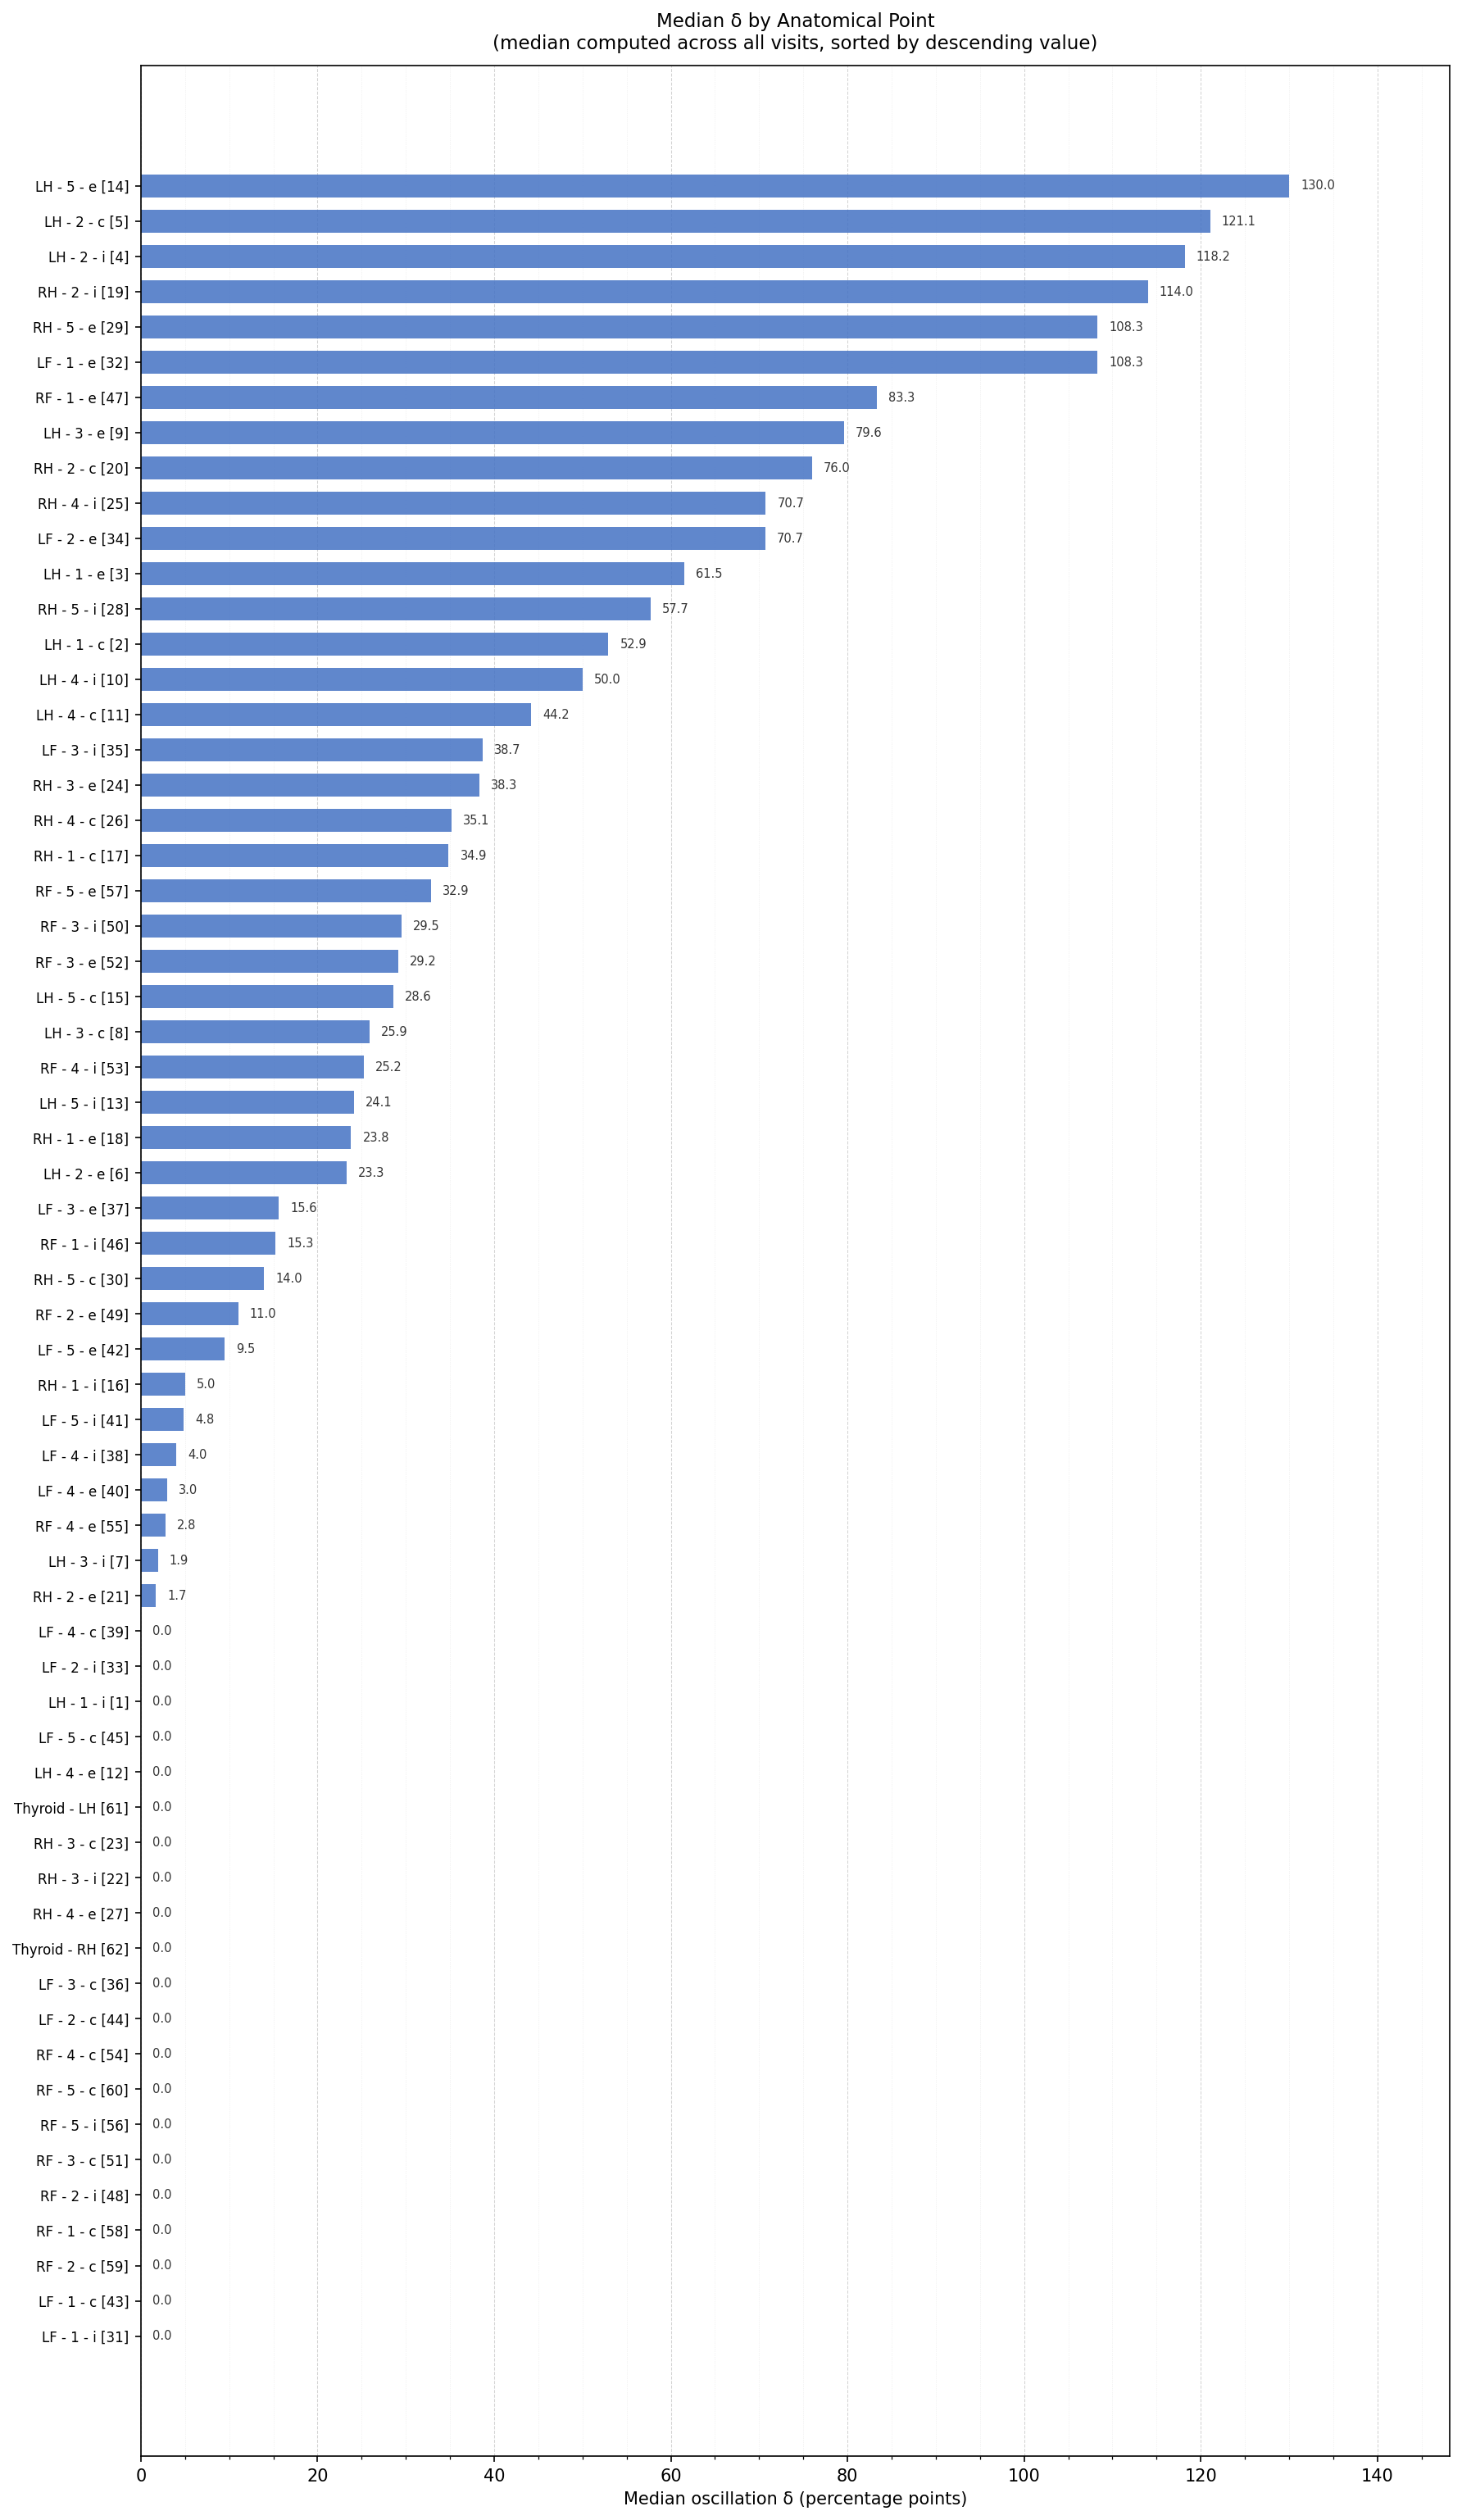
\includegraphics[width=\textwidth,height=0.92\textheight,keepaspectratio]{figures/median_by_point.png}
  \caption{Median $\delta$ per anatomical point, sorted descending.
    Each bar represents the median of all oscillation values computed
    for that point across all visits.
    Values are in percentage points (pp).}
  \label{fig:median_by_point}
\end{figure}

\newpage

%%--------------------------------------------------------------
\section{Median \texorpdfstring{$\delta$}{delta} per Point --- Full Table}
%%--------------------------------------------------------------

The following table reports the exact median $\delta$ (in percentage points)
for each of the 62 anatomical points, sorted in descending order.
The values are identical to those displayed in Figure~\ref{fig:median_by_point}
and are provided here for precise reading and comparison.

\bigskip

\begin{longtable}{@{}rlr@{}}
\toprule
\textbf{Rank} & \textbf{Anatomical Point} & \textbf{Median $\delta$ (pp)} \\
\midrule
\endfirsthead
\multicolumn{3}{l}{\small\itshape (continued from previous page)} \\
\toprule
\textbf{Rank} & \textbf{Anatomical Point} & \textbf{Median $\delta$ (pp)} \\
\midrule
\endhead
\midrule
\multicolumn{3}{r}{\small\itshape (continued on next page)} \\
\endfoot
\bottomrule
\endlastfoot
    1 & LH - 5 - e [14] & 130.00 \\
    2 & LH - 2 - c [5] & 121.05 \\
    3 & LH - 2 - i [4] & 118.18 \\
    4 & RH - 2 - i [19] & 114.00 \\
    5 & RH - 5 - e [29] & 108.33 \\
    6 & LF - 1 - e [32] & 108.33 \\
    7 & RF - 1 - e [47] & 83.33 \\
    8 & LH - 3 - e [9] & 79.62 \\
    9 & RH - 2 - c [20] & 76.00 \\
    10 & RH - 4 - i [25] & 70.74 \\
    11 & LF - 2 - e [34] & 70.71 \\
    12 & LH - 1 - e [3] & 61.54 \\
    13 & RH - 5 - i [28] & 57.69 \\
    14 & LH - 1 - c [2] & 52.94 \\
    15 & LH - 4 - i [10] & 50.00 \\
    16 & LH - 4 - c [11] & 44.17 \\
    17 & LF - 3 - i [35] & 38.71 \\
    18 & RH - 3 - e [24] & 38.30 \\
    19 & RH - 4 - c [26] & 35.15 \\
    20 & RH - 1 - c [17] & 34.85 \\
    21 & RF - 5 - e [57] & 32.88 \\
    22 & RF - 3 - i [50] & 29.47 \\
    23 & RF - 3 - e [52] & 29.17 \\
    24 & LH - 5 - c [15] & 28.57 \\
    25 & LH - 3 - c [8] & 25.86 \\
    26 & RF - 4 - i [53] & 25.23 \\
    27 & LH - 5 - i [13] & 24.14 \\
    28 & RH - 1 - e [18] & 23.81 \\
    29 & LH - 2 - e [6] & 23.33 \\
    30 & LF - 3 - e [37] & 15.65 \\
    31 & RF - 1 - i [46] & 15.25 \\
    32 & RH - 5 - c [30] & 13.96 \\
    33 & RF - 2 - e [49] & 11.03 \\
    34 & LF - 5 - e [42] & 9.52 \\
    35 & RH - 1 - i [16] & 5.00 \\
    36 & LF - 5 - i [41] & 4.84 \\
    37 & LF - 4 - i [38] & 4.03 \\
    38 & LF - 4 - e [40] & 2.99 \\
    39 & RF - 4 - e [55] & 2.78 \\
    40 & LH - 3 - i [7] & 1.93 \\
    41 & RH - 2 - e [21] & 1.68 \\
    42 & LF - 2 - c [44] & 0.00 \\
    43 & LF - 2 - i [33] & 0.00 \\
    44 & LF - 3 - c [36] & 0.00 \\
    45 & LF - 4 - c [39] & 0.00 \\
    46 & LF - 5 - c [45] & 0.00 \\
    47 & LH - 4 - e [12] & 0.00 \\
    48 & LH - 1 - i [1] & 0.00 \\
    49 & LF - 1 - i [31] & 0.00 \\
    50 & LF - 1 - c [43] & 0.00 \\
    51 & RF - 2 - c [59] & 0.00 \\
    52 & RF - 1 - c [58] & 0.00 \\
    53 & RF - 2 - i [48] & 0.00 \\
    54 & RF - 3 - c [51] & 0.00 \\
    55 & RF - 5 - i [56] & 0.00 \\
    56 & RF - 5 - c [60] & 0.00 \\
    57 & RF - 4 - c [54] & 0.00 \\
    58 & RH - 3 - c [23] & 0.00 \\
    59 & RH - 3 - i [22] & 0.00 \\
    60 & RH - 4 - e [27] & 0.00 \\
    61 & Thyroid - LH [61] & 0.00 \\
    62 & Thyroid - RH [62] & 0.00 \\
\end{longtable}

\end{document}
